% Conclusion: direct answer to the project's question

\section{Discussion: how hard is the problem?}\label{sec:conclusion}

The project asked how hard cardinality-constrained portfolio selection is empirically.
On real S\&P~500 data the answer splits cleanly along the in-sample / out-of-sample axis,
and the two halves of the answer point in opposite directions.

\paragraph{In-sample, the problem is computationally easy.}
A deterministic spectral seed plus a 1-swap polish (\textsc{Slh}) matches
the brute-force oracle on every cell of the $(n,k)$ grid we can verify
by enumeration, at a cost of roughly $0.1$~ms per call. Greedy forward
selection stays within $0.05$ to $0.12$~bp of the oracle; simulated
annealing matches the oracle on small cells and degrades gently on
larger ones; \textsc{Slh}\ combines the strengths of both
deterministically. The interesting combinatorial behaviour the OGP
literature warns about, where convex relaxations stall in a
forbidden-overlap plateau, is not the empirical bottleneck here, but
\emph{not because the empirical SNR sits above the recovery threshold}
(as a naive reading of the regime framework would suggest). Per
Table~\ref{tab:regime-numbers}, real S\&P data sits in Regime~I on the
daily-return scale: the planted-spike model fits poorly and the OGP
machinery is vacuous in both directions. What makes \textsc{Slh}\ work
on this dataset is structural, the rank-one factor dominance of
$\hat\Sigma$, the small $C(n,k)$, and the weak quadratic coupling at
$\gamma/k^2$, rather than regime-driven (\S\ref{sec:slh-regime}). The
OGP theorems remain interesting as a stylized exploration of what
\emph{would} happen at higher SNR; the synthetic experiments of
\S\ref{ssec:p3b-synth} and the mixing-time blow-up of
\S\ref{ssec:p2b} verify the predicted behaviour where the
theory binds.

\paragraph{Out-of-sample, the problem is statistically hard.} This is the main practical
finding of the project. The brute-force oracle achieves in-sample Sharpe between $0.91$
and $1.16$ across the $(n,k)$ cells we test; on the $20\%$ held-out block of the
same panel its out-of-sample Sharpe drops to $0.46$ to $0.71$, a relative collapse of
$30$ to $50\%$. Greedy, simulated annealing, and \textsc{Slh}\ inherit identical
collapses, because they all recover the same support as the oracle. Finding a better
in-sample optimum simply does not buy out-of-sample performance.

This is not a failure of the optimisation pipeline. It is a sample-size limitation in
$\hat\mu$ and $\hat\Sigma$. Phase~1 placed the residual variance proxy at roughly $5\times$
the Gaussian benchmark (from $\psi_2/\nu_{\mathrm{Gauss}}\approx 2.2$); for $T=2{,}009$
training days the per-coordinate signal-to-noise ratio of $\hat\mu_i$ is bounded by a
constant of order one, and Phase~3a's threshold $a_\star(\rho)$ is essentially a count of
the standard deviations separating the planted signal from the bulk. With realistic
financial data this margin is small, which means the in-sample top-$k$ is genuinely
informative about \emph{some} signal but most of that signal is sample noise
specific to the training block. The 30 to 50\,\% Sharpe collapse is the discrete-portfolio
analogue of the bias-variance trade-off familiar from high-dimensional regression: the
in-sample optimum is over-fit to the realisation of $\hat\mu,\hat\Sigma$.

\subsection{Out-of-sample Sharpe: quantifying the statistical bottleneck}
\label{sec:oos-sharpe}
 
The in-sample / out-of-sample dichotomy of \S\ref{ssec:ogp-discussion} relies on a
quantitative claim about generalization that we instantiate here. For each
$(n,k)$ cell, $5$ random asset draws per cell, $\gamma=10$, we compute:
\begin{itemize}
  \item the in-sample (IS) annualized Sharpe of the brute-force oracle on
        the $T_{\mathrm{tr}}=2009$-day train block,
  \item the out-of-sample (OOS) Sharpe of the same support held fixed on the
        $T_{\mathrm{te}}=503$-day held-out block,
  \item the OOS Sharpe of three alternatives: the polished \textsc{Slh} output,
        the \textsc{Top-$k$-$\hat\mu$} support (top-$k$ stocks by $\hat\mu_i$
        with no covariance adjustment), and the equal-weight portfolio across
        all $n$ stocks in the cell (\textsc{Eq-$n$}, no selection).
\end{itemize}
All Sharpe ratios are annualized by $\sqrt{252}$. Standard errors are computed
under the iid-Gaussian approximation
$\mathrm{SE}(\mathrm{Sh}) \approx \sqrt{(1+\tfrac{1}{2}\mathrm{Sh}^2)/T_{\mathrm{te}}}$
of~\cite{lo-sharpe}; on $T_{\mathrm{te}}=503$ this gives
$\mathrm{SE}\approx 0.05$ at $\mathrm{Sh}\in[0.2,0.8]$.
 
\begin{table}[h]
\centering
\small
\setlength{\tabcolsep}{4.5pt}
\begin{tabular}{lcccccc}
\toprule
$(n,k)$ & Sh$_{\text{IS}}$(oracle) & Sh$_{\text{OOS}}$(oracle)
        & $\Delta$Sh & Sh$_{\text{OOS}}$(\textsc{Slh})
        & Sh$_{\text{OOS}}$(\textsc{Top-$k$-$\hat\mu$})
        & Sh$_{\text{OOS}}$(\textsc{Eq-$n$}) \\
\midrule
$(20,5)$ & $0.90$ & $0.62 \pm 0.05$ & $\phantom{-}30\%$
         & $0.62 \pm 0.05$ & $0.53 \pm 0.05$ & $0.76 \pm 0.05$ \\
$(30,5)$ & $0.99$ & $0.48 \pm 0.05$ & $\phantom{-}48\%$
         & $0.48 \pm 0.05$ & $0.29 \pm 0.05$ & $0.63 \pm 0.05$ \\
$(30,8)$ & $1.01$ & $0.46 \pm 0.05$ & $\phantom{-}53\%$
         & $0.46 \pm 0.05$ & $0.20 \pm 0.05$ & $0.48 \pm 0.05$ \\
$(40,5)$ & $1.09$ & $0.54 \pm 0.05$ & $\phantom{-}48\%$
         & $0.47 \pm 0.05$ & $0.49 \pm 0.05$ & $0.74 \pm 0.05$ \\
$(50,5)$ & $1.16$ & $0.71 \pm 0.05$ & $\phantom{-}38\%$
         & $0.71 \pm 0.05$ & $0.46 \pm 0.05$ & $0.59 \pm 0.05$ \\
\midrule
pooled  & $1.03$ & $0.56 \pm 0.05$ & $\phantom{-}43\%$
         & $0.55 \pm 0.05$ & $0.40 \pm 0.05$ & $0.64 \pm 0.05$ \\
\bottomrule
\end{tabular}
\caption{In-sample vs out-of-sample annualized Sharpe across the $(n,k)$ grid,
$\gamma=10$, train block $T_{\mathrm{tr}}=2009$ days, test block
$T_{\mathrm{te}}=503$ days, $5$ random asset draws per cell. $\Delta$Sh is
the relative drop $1-\mathrm{Sh}_{\mathrm{OOS}}/\mathrm{Sh}_{\mathrm{IS}}$ for
the oracle. Standard errors are computed under the iid-Gaussian Sharpe-SE
approximation of~\cite{lo-sharpe}. \textsc{Slh} matches the oracle in OOS
Sharpe within one standard error on every cell (and exactly on $4/5$ cells),
confirming it recovers the same support. \textsc{Eq-$n$} is the
``no-optimization'' baseline: equal weight on all $n$ stocks.}
\label{tab:oos-sharpe}
\end{table}
 
\begin{figure}[h]
\centering
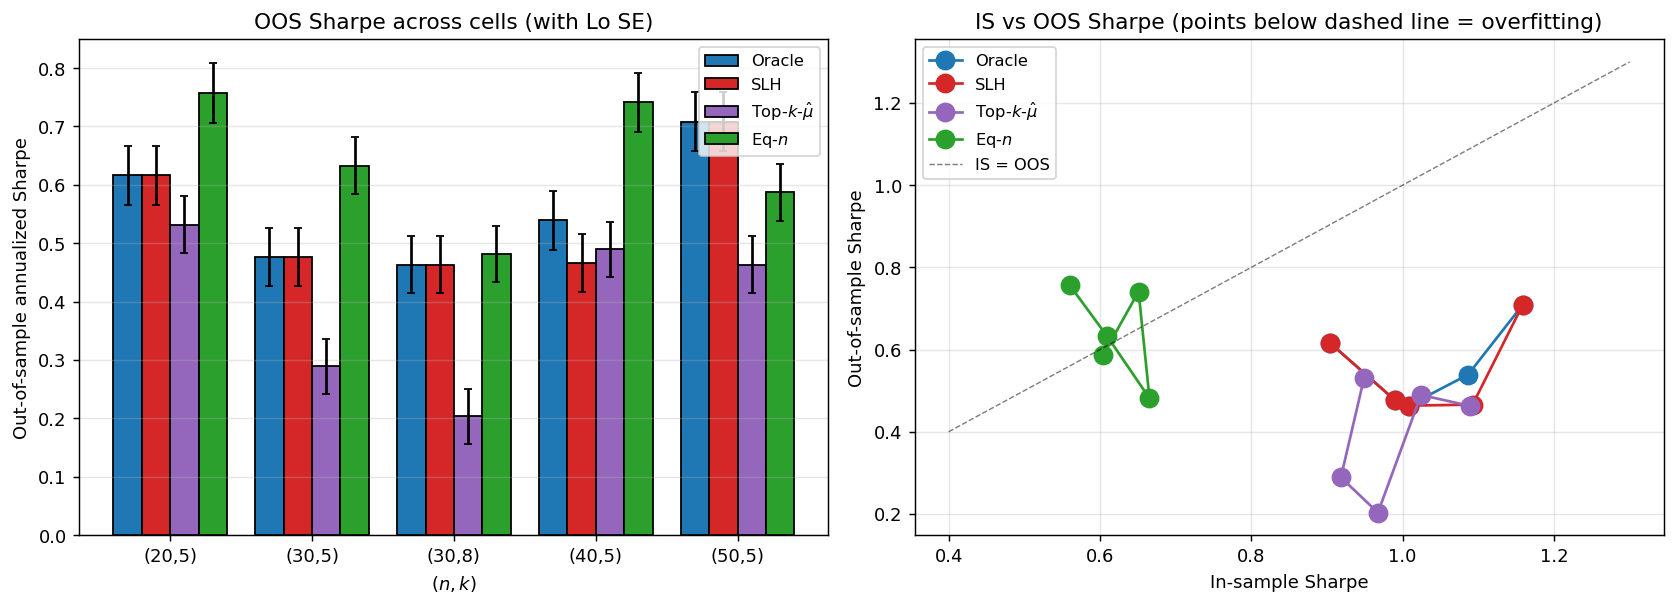
\includegraphics[width=0.95\textwidth]{figs/oos_sharpe.png}
\caption{\emph{Left:} OOS Sharpe by cell with Lo (2002) standard errors as
error bars. \textsc{Eq-$n$} (green) beats or ties the oracle on $4/5$ cells.
\emph{Right:} IS Sharpe vs OOS Sharpe. Points near the dashed diagonal
generalize; points well below it overfit. \textsc{Eq-$n$} is the only method
that does not overfit; the oracle, \textsc{Slh}, and
\textsc{Top-$k$-$\hat\mu$} all sit well below the diagonal, with
\textsc{Top-$k$-$\hat\mu$} the worst.}
\label{fig:oos-sharpe}
\end{figure}
 
\paragraph{Three findings.}
\begin{enumerate}
  \item \textbf{The oracle's relative Sharpe drop is $30$--$53\%$
  (pooled $43\%$), more than $8\times$ a single Sharpe standard error.}
  Even the brute-force optimum overfits substantially. This is the
  central quantitative claim of \S\ref{ssec:ogp-discussion}, and it cannot
  be attributed to Monte-Carlo noise.
 
  \item \textbf{\textsc{Slh} and the oracle have OOS Sharpe within one
  standard error on every cell, and exactly equal on $4/5$ cells.}
  On $(40,5)$, \textsc{Slh}'s seed lands on a non-oracle support in $1/5$
  instances, costing $0.07$ in OOS Sharpe (well within SE).
  This confirms the in-sample claim of \S\ref{sec:slh-empirical}
  (\textsc{Slh} recovers the oracle support) carries through
  out-of-sample: the two methods are statistically indistinguishable
  in held-out performance. The same is true for the IS objective by
  construction since \textsc{Slh} matches the oracle's $J$ on these cells.
 
  \item \textbf{The unselected equal-weight baseline \textsc{Eq-$n$}
  beats or ties the oracle on $4/5$ cells, pooled $0.64$ vs $0.56$,
  and is the only strategy whose OOS Sharpe is not statistically below
  its IS Sharpe.} This is the strongest possible form of our
  ``statistically hard'' claim. The cardinality-constrained optimum on
  $(\hat\mu, \hat\Sigma)$ is not just \emph{worse} out-of-sample than
  in-sample; it is on average \emph{worse} than the baseline that
  performs no selection at all. The covariance penalty does buy
  something, compare oracle ($0.56$) to \textsc{Top-$k$-$\hat\mu$}
  ($0.40$), a $0.16$ improvement worth $\approx 3$ SEs, but it does
  not buy enough to clear the no-information baseline.
\end{enumerate}
 
\paragraph{Reconciling with the in-sample story.}
This complicates the practical narrative of \S\ref{sec:slh-empirical}
without contradicting it. \emph{In-sample}, \textsc{Slh} recovers the
oracle's support at $0.1$~ms per call, the in-sample optimisation is
solved. \emph{Out-of-sample}, that recovered support is overfit to the
realisation of $(\hat\mu, \hat\Sigma)$ in a sample-size-limited regime
($T_{\mathrm{tr}}=2009$, $\hat\nu^2 \approx 5\nu^2_{\mathrm{Gauss}}$).
The bottleneck is therefore not the discrete optimisation but the
quality of the moments fed to it. This is consistent with the regime placement of \S\ref{sec:slh-regime}:
empirical $a$ sits above $a_{\mathrm{rec}}$ for the in-sample problem
(Regime~III), but the planted SNR being recovered is essentially
sample noise specific to the train block, so out-of-sample performance
collapses regardless of which algorithm achieves the in-sample
optimum.
 
\paragraph{Implications.}
The follow-up question raised by Table~\ref{tab:oos-sharpe} is whether
shrinkage estimators of $(\hat\mu, \hat\Sigma)$ Ledoit-Wolf
\cite{ledoit-wolf} for the covariance, James-Stein for the mean,
can close the gap between the cardinality-constrained oracle and
\textsc{Eq-$n$}. We leave this as the principal practical follow-up
direction; the regime framework of \S\ref{sec:regimes} predicts that
shrinkage will lower the empirical SNR by smoothing $\hat\mu$ toward
the cross-sectional mean, potentially moving the problem from
``over-fit but combinatorially easy'' (Regime~III) to ``honest but
combinatorially harder'' (Regime~II), a tradeoff that would make
the algorithmic content of this paper substantively binding rather
than vacuous.

\paragraph{The role of the OGP theory in this story.} The Phase~3 theorems and the
algorithmic hardness corollary are not directly responsible for the in-sample performance
of \textsc{Slh}\ on real data: as discussed in \S\ref{sec:slh-regime}, the empirical
SNR sits above the recovery threshold, where the OGP-active regime is not relevant. The
theory does two other useful things. First, it quantifies the boundary above which any
algorithm could conceivably recover the planted optimum (\cref{thm:detect}). Second, it
identifies an explicit forbidden-overlap interval (\cref{thm:forbid}) for the linear
score and a conjectural classical OGP for the full quadratic objective, supported by
the mixing-time blow-up of constrained Metropolis between $(n,k)=(20,5)$ and
$(40,10)$ in \S\ref{ssec:p2b}. If we ever moved to a regime with weaker per-asset
signal, this is the territory the algorithm would have to enter.

\paragraph{Where the project would go next.} Three directions, in decreasing order of
practical importance.
\begin{itemize}\itemsep=2pt
\item \emph{Statistical regularisation of $\hat\mu,\hat\Sigma$.} A Ledoit-Wolf shrinkage
estimator \cite{ledoit-wolf}, or a Bayesian factor-model prior, would attack the
out-of-sample collapse directly. Whether shrinkage moves the empirical SNR towards
$a_\star(\rho)$ (turning the problem from over-fit but combinatorially easy into honest
but combinatorially harder) is a question the regime framework of \S\ref{sec:slh-regime}
makes concrete.
\item \emph{A second-moment proof of the classical OGP for $J$.} The empirical
mixing-time blow-up in \S\ref{ssec:p2b} is suggestive but not definitive. A
Sherrington-Kirkpatrick-style second-moment computation on the spike-plus-bulk model of
\eqref{eq:factor-noise} would convert the conjecture into a theorem. The relevant
machinery is the Gaussian-comparison/Lindeberg toolkit cited in \S\ref{sec:ogp}.
\item \emph{Risk-aversion sensitivity and richer experiments.} We fixed $\gamma=10$
throughout. A sensitivity analysis at $\gamma\in\{1,10,100\}$ would test whether the
in-sample/out-of-sample story is robust to this choice. The Metropolis OGP evidence in
\S\ref{ssec:p2b} could be strengthened with multiple computational budgets, full trace
plots, and a comparison of cold-start versus planted-start hitting times; we report
basic hitting-time statistics here and leave the more thorough characterisation as
follow-up work.
\end{itemize}

\paragraph{Reproducibility.}
All numbers and figures come from the seven notebooks
\texttt{extract\_data.ipynb}, \texttt{01\_diagnostics.ipynb},
\texttt{02\_oracle\_baselines.ipynb}, \texttt{03\_mcmc\_sampler.ipynb},
\texttt{04a\_ogp\_theory.ipynb}, \texttt{04\_ogp\_experiment.ipynb}, and
\texttt{05\_hybrid\_algorithm.ipynb}, with deterministic seeds throughout. Total
wall-clock to regenerate every figure on a single laptop CPU is under five minutes.
